%=== CHAPTER ONE (1) ===
%=== INTRODUCTION ===

\chapter{Introduction}
\begin{spacing}{1.5}
\setlength{\parskip}{0.3in}

The first chapter of the dissertation is almost invariably the Introduction. Generally, its purpose is to lead the readers into the problem you intend to attack in the project, to set the scene. The main points here consist of the background to the problem and your motivation in solving it. This then leads into the objectives and the scope of the project. It is good to conclude your Introduction with a section on the layout of the dissertation. It prepares the readers for what is to come

\section{Background}


Background goes here. Also you can put in some references~\cite{ronneberger2015unet}.

Here is a sample of table in \autoref{tabelsample}

\begin{table}[ht]
\centering
\caption{A table without vertical lines.}
\label{tabelsample}
\begin{tabular}[t]{lcc}
\toprule
&Treatment A&Treatment B\\
\midrule
John Smith&1&2\\
Jane Doe&--&3\\
Mary Johnson&4&5\\
\bottomrule
\end{tabular}
\end{table}%

Use  \texttt{$\backslash$newpage} to force start a new page.

\newpage

Also can try to refer to this image in \autoref{fig:boundingboxexample}. Notice that the \texttt{.eps} and \texttt{.pdf} format vector graphs are favoured, because:

\begin{enumerate}
    \item they can be zoomed-in to check the detail.
    \item text in such formats are search-able.
\end{enumerate}


\begin{figure}[ht]
\centering
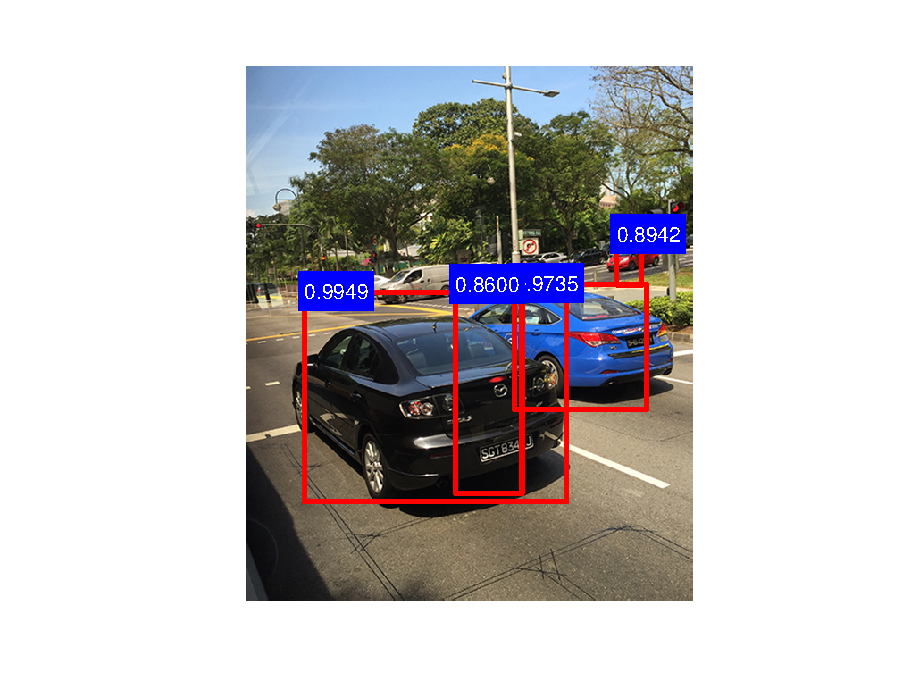
\includegraphics[width=4in, fbox]{Chapter1/boundingbox.eps}
\caption{Bounding-box example of cars.}
\label{fig:boundingboxexample} 
\end{figure}

Try to insert a math equation as in \autoref{eq:euler}. If you wanna try the in-line mathematical, here is a sample $\alpha = \pi \cdot \frac{1}{\Theta}$.

\begin{equation}
\label{eq:euler}
    e^{ix}= \cos{x} + i \sin{x}
\end{equation}

Also here is a sample for footnote and hyperlink url\footnote{\url{https://github.com/doem97}}.

When mention some file formats can use \texttt{music.mp3}, \texttt{latex.pdf}, etc.

If there are any update of the dissertation standard, or you want to contribute to the \texttt{NTU-EEE-MSc-Dissertation-Template} project too, kindly send an E-mail to me. Thank you :)

\section{Motivation}


\section{Objectives and Specifications}



\section{Major contribution of the Dissertation}



\section{Organisation of the Dissertation}


\end{spacing}
%=== END OF CHAPTER ONE ===
\newpage


